\section{Results}
\label{sec:results}

\subsection{Bandwidth metrics and cost model}
\label{sec:cost-model}

Following the convention \texttt{nccl-tests} itself uses \citep{nvidia2024ncclperf}, since this project explicitly mirrors NCCL's ring transport, two bandwidth figures are computed from every timed measurement. Algorithm bandwidth is the simple ratio $\text{algbw} = M / T$ of message size to elapsed time. Bus bandwidth rescales it by $\text{busbw} = \text{algbw} \cdot \frac{2(N-1)}{N}$, the ratio of bytes actually moved over the network to bytes of input, for any bandwidth-optimal point-to-point allreduce regardless of whether its underlying algorithm is a ring, a tree, or something else \citep{nvidia2024ncclperf}. Because that factor is baked in, busbw is comparable across different process counts against one single hardware bandwidth ceiling, which algbw alone is not.

That ceiling is estimated from this project's own data, not assumed. The Hockney latency-bandwidth model,
\begin{equation}
  T(N, M) \approx 2(N-1)\,\alpha \;+\; 2\,\frac{N-1}{N}\,M\,\beta,
  \label{eq:hockney}
\end{equation}
gives $\alpha$ (seconds of fixed per-message latency) and $\beta$ (seconds per byte, i.e. inverse bandwidth) as the two free parameters, fit independently for each algorithm variant by weighted least squares against that variant's own measured $(N, M, T)$ triples (\texttt{analysis/theoretical\_model.py}). The fit is weighted by $1/T$, turning it into a relative rather than absolute error minimization: this project's sweep spans roughly seven orders of magnitude in message size and therefore in $T$, and an unweighted fit is so dominated by the handful of largest, slowest configurations that $\alpha$, whose entire contribution to $T$ is only visible at the smallest sizes, comes out badly biased even though $\beta$ and the overall $R^2$ both look excellent. That failure mode was demonstrated rather than assumed. Showing that a fitter recovers the right answer requires already knowing the right answer, which real measurements do not come with, so the procedure is verified against data synthesized from known constants, in the same spirit as checking a numerical solver against a manufactured solution. That check is \texttt{analysis/validate\_fit.py}, and it is reproducible: across its cases, unweighted least squares recovers $\beta$ to within a fraction of a percent but misses $\alpha$ by as much as 17\%, while the $1/T$-weighted fit recovers both to within 0.4\%. That validated weighted fit is what is applied to the real measurements below. Theoretical peak bus bandwidth is reported as $1/\beta$, and efficiency at a given configuration as achieved busbw divided by that peak.

Table~\ref{tab:fits} gives the fitted constants. One property of the fit on this hardware needs stating up front, because it shapes how the figures should be read. On a single node the transport is shared memory, and its effective per-byte cost is not the single constant Equation~\ref{eq:hockney} assumes: a reduction whose working set fits in the 33~MB L3 cache moves bytes considerably faster than one large enough to be bound by main-memory bandwidth. A single straight-line fit across the full 8~B to 128~MiB range therefore has genuinely limited explanatory power here, with $R^2$ between 0.28 and 0.33 for the three variants. The fitted $1/\beta$ is best read not as a hard ceiling but as a sustained-bandwidth average over the whole size range; as the next figures show, the fastest cache-resident sizes exceed it, which is a real feature of single-node shared-memory transport rather than a fitting error. A network-fabric multi-node sweep would be expected to track the linear model far more closely.

\begin{table}[htbp]
\centering
\begin{tabular}{lrrrr}
\toprule
Algorithm & $\alpha$ ($\mu$s) & $\beta$ (ns/byte) & $1/\beta$ (GB/s) & $R^2$ \\
\midrule
custom ring              & 0.264 & 0.1241 & 8.06 & 0.28 \\
\texttt{MPI\_Allreduce}, default     & 0.090 & 0.1737 & 5.76 & 0.30 \\
\texttt{MPI\_Allreduce}, forced ring & 0.113 & 0.1514 & 6.61 & 0.33 \\
\bottomrule
\end{tabular}
\caption{Hockney constants fit from this project's own measurements, per algorithm variant. The custom ring has the \emph{worst} per-message latency $\alpha$ but the \emph{best} inverse bandwidth $\beta$, and therefore the highest sustained-bandwidth asymptote $1/\beta$: it is slower to start a step and faster to move bytes once started. Section~\ref{sec:discussion} takes up why.}
\label{tab:fits}
\end{table}

\subsection{Achieved bus bandwidth versus message size}

Figure~\ref{fig:busbw-vs-size} plots achieved busbw against message size for a representative subset of process counts, one panel per algorithm variant, with each panel's fitted $1/\beta$ as a dashed reference. All three variants share the same three-part shape, and it is more interesting than a simple climb to a plateau. At small message sizes busbw sits in a flat, near-zero floor where the fixed per-step latency dominates and the payload is too small to matter. It then climbs steeply and, on this single node, keeps climbing past the fitted $1/\beta$ line to a pronounced peak in the hundreds-of-kilobytes to low-megabyte range, where the working set is still L3-cache-resident: all three variants peak at close to 16~GB/s at $N=2$ (the custom ring at 16.1~GB/s near 512~KiB, both vendor variants at 16.0~GB/s near 1~MiB), well above their own sustained-bandwidth asymptotes. Past that peak busbw falls again as the buffers outgrow cache and the reduction becomes bound by main-memory bandwidth, which is exactly why a single-slope fit reports the modest $R^2$ of Table~\ref{tab:fits}.

\begin{figure}[htbp]
\centering
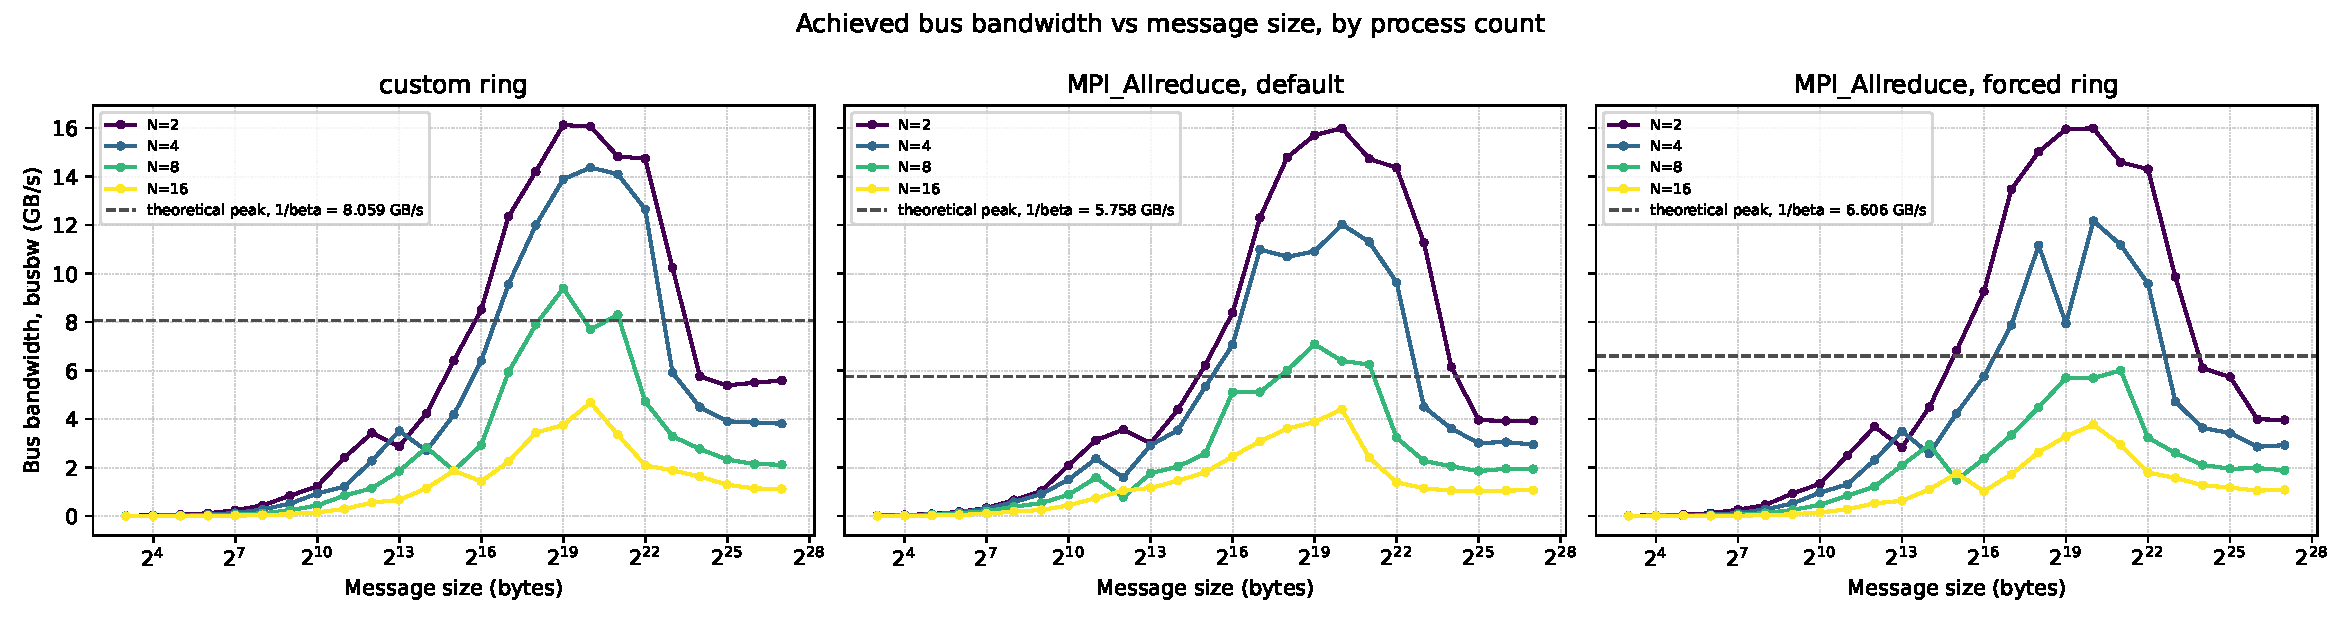
\includegraphics[width=\textwidth]{figures/busbw_vs_size.pdf}
\caption{Achieved bus bandwidth versus message size, log-scaled on the size axis, for $N \in \{2,4,8,16\}$, one panel per algorithm variant. The dashed line in each panel is that variant's fitted theoretical peak, $1/\beta$.}
\label{fig:busbw-vs-size}
\end{figure}

Table~\ref{tab:summary} quotes the two ends of the sweep at $N=16$, the most demanding process count. At 8~bytes every variant sits at a small fraction of a percent of its fitted peak, the latency-bound floor. At 128~MiB, the memory-bound far end, the custom ring reaches the highest absolute bus bandwidth of the three (1.120~GB/s, against 1.083 for the forced vendor ring and 1.070 for the default selection), though as a percentage of its own higher fitted asymptote that is a smaller fraction.

\begin{table}[htbp]
\centering
\begin{tabular}{lrrrr}
\toprule
Algorithm & busbw @ 8B (GB/s) & \% peak & busbw @ 128MiB (GB/s) & \% peak \\
\midrule
ring & 0.0013 & 0.02 & 1.120 & 13.90 \\
mpi-default & 0.0066 & 0.12 & 1.070 & 18.58 \\
mpi-ring & 0.0070 & 0.11 & 1.083 & 16.39 \\
\bottomrule
\end{tabular}

\caption{Achieved busbw and percent of that variant's fitted theoretical peak at the smallest (8~B) and largest (128~MiB) swept message sizes, at $N=16$: the most demanding process count in the sweep and therefore the most informative single configuration to summarize (averaging across $N$ would blend together regimes with very different busbw at the same message size and would not describe any one real configuration).}
\label{tab:summary}
\end{table}

\subsection{The head-to-head: two different comparisons}
\label{sec:head-to-head}

The central experimental result is not a single winner but the difference between two comparisons, which is exactly what benchmarking against both vendor variants (Section~\ref{sec:mca-forcing}) was designed to expose. Table~\ref{tab:headtohead} shows median times at $N=16$ across the size range.

\begin{table}[htbp]
\centering
\begin{tabular}{rrrr}
\toprule
Message size & custom ring ($\mu$s) & default ($\mu$s) & forced ring ($\mu$s) \\
\midrule
8~B      & 11.55     & 2.26      & 2.16 \\
64~B     & 11.08     & 2.41      & 11.97 \\
4~KiB    & 13.74     & 7.29      & 14.54 \\
64~KiB   & 85.72     & 49.86     & 119.21 \\
1~MiB    & 419.67    & 446.33    & 521.03 \\
16~MiB   & 19243.90  & 29920.40  & 24616.60 \\
128~MiB  & 224656.00 & 235199.00 & 232361.00 \\
\bottomrule
\end{tabular}
\caption{Median completion time at $N=16$ (lower is better). Against the \emph{default} selection the custom ring is roughly five times slower at 8~B and only overtakes it around 1~MiB. Against Open~MPI's \emph{own ring}, forced via MCA, the custom ring tracks it almost exactly from 64~B onward and beats it from 64~KiB up. The two rings behaving alike, while the default behaves entirely differently, is the step-count argument of Section~\ref{sec:step-count} measured directly.}
\label{tab:headtohead}
\end{table}

Against the default selection, the custom ring loses badly at small messages: 11.55~$\mu$s versus 2.26~$\mu$s at 8~bytes, a factor of roughly five, and it does not overtake the default until around 1~MiB. Against Open~MPI's own ring algorithm, the picture is completely different. From 64~bytes upward the forced vendor ring costs 11.97~$\mu$s at $N=16$ while the custom ring costs 11.08~$\mu$s: the two implementations of the same algorithm sit within about 8\% of each other, both roughly five times slower than the default selection. From 64~KiB upward the custom ring is the faster of the two rings, and by 16~MiB it completes in 19.2~ms against the vendor ring's 24.6~ms.

The one place the two rings diverge is at the very smallest sizes, 8~B and 32~B, where the forced vendor ring is as fast as the default selection rather than ring-like. The most likely explanation is that Open~MPI's tuned component retains a short-message special case that the MCA forcing does not fully override; the honest statement is that from 64~bytes upward, where the forcing demonstrably does take effect, the two rings behave like the same algorithm, because they are.

\subsection{Efficiency across the full sweep}

Figure~\ref{fig:efficiency-heatmap} extends this across every swept $(N, M)$ combination at once, with efficiency defined as achieved busbw over the fitted $1/\beta$ and the color scale allowed to run past 1 so the cache-resident band is not clipped away. The pattern is consistent across all three variants: efficiency is near zero across the small-message columns regardless of $N$, where the latency term of Equation~\ref{eq:hockney} dominates; it then rises through a bright band above the $1/\beta$ reference at the cache-resident middle sizes; and it falls back below 1 at the memory-bound largest sizes. The message size at which efficiency first lifts off the floor shifts right, toward larger messages, as $N$ grows, exactly as Equation~\ref{eq:hockney} predicts: the latency term scales with $N-1$, so more of the size axis stays latency-bound at larger $N$.

\begin{figure}[htbp]
\centering
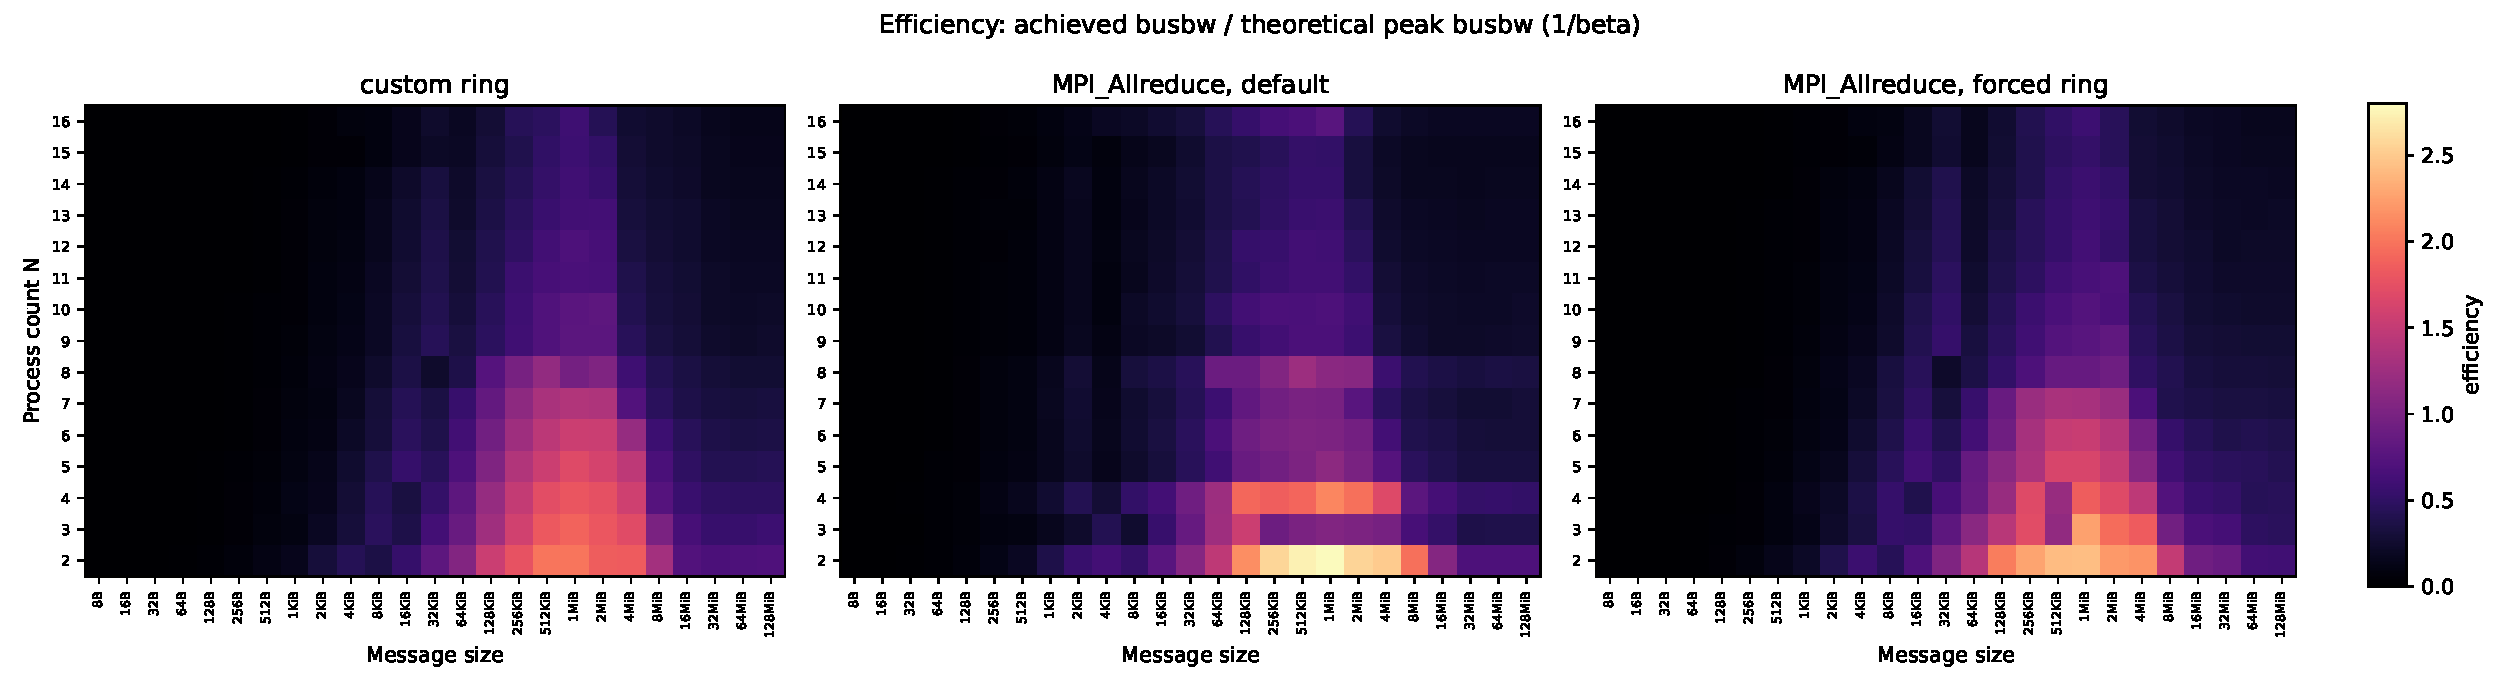
\includegraphics[width=\textwidth]{figures/efficiency_heatmap.pdf}
\caption{Efficiency (achieved busbw divided by that variant's fitted theoretical peak) across every swept process count and message size, one panel per algorithm variant. Values above 1 are the cache-resident sizes that beat the full-range sustained-bandwidth average, not a violation of the model.}
\label{fig:efficiency-heatmap}
\end{figure}

\subsection{Decomposing the latency floor}

Figure~\ref{fig:latency-decomposition} isolates the smallest swept message size and, for the custom ring specifically, breaks the cost model's prediction into its two additive terms per process count, alongside both the measured time and a raw \texttt{MPI\_Send}/\texttt{MPI\_Recv} ping-pong one-way latency taken on the same hardware in the same run (\texttt{apps/pingpong}, using the same one-way-latency-from-round-trip convention as OSU Micro-Benchmarks' \texttt{osu\_latency} \citep{osu2024benchmarks}).

Three things are visible at once. First, the bandwidth term is not merely small but numerically irrelevant: at 8~bytes it never exceeds $0.0019~\mu$s against a latency term of several microseconds, so at this size $T$ is the latency term and nothing else. Second, the raw ping-pong one-way latency is \textbf{0.1585~$\mu$s}, so a ring whose every step cost exactly one bare point-to-point message would take $2(N-1) \times 0.1585~\mu$s: that is the dashed "ideal floor" line, the best any ring could do on this hardware. Third, and most usefully, the measured time sits \emph{on} that floor for most of the range. Up to about $N=14$ the custom ring's measured 8-byte time tracks the ideal floor closely, meaning its per-step cost really is close to a bare point-to-point send and there is very little synchronization overhead to speak of.

The exception is the top of the range. At $N=15$ and $N=16$ the measured time jumps well above the floor, reaching 11.55~$\mu$s at $N=16$ against a floor of 4.7~$\mu$s. The shaded region in Figure~\ref{fig:latency-decomposition} is that excess, and it is the rank-synchronization overhead made visible: it is small and roughly flat while ranks are cheap to schedule, and it grows abruptly once they are not. A likely cause on this specific CPU is its hybrid topology (8 performance cores, each with two hardware threads, plus 12 efficiency cores): past a certain rank count the ring's slowest participant, which is what \texttt{MPI\_MAX} across ranks selects, starts landing on a hardware thread that shares execution resources with a sibling, or on a slower core, and every one of the $2(N-1)$ steps then waits on that straggler. Section~\ref{sec:discussion} takes up what this means and what it does not.

\begin{figure}[htbp]
\centering
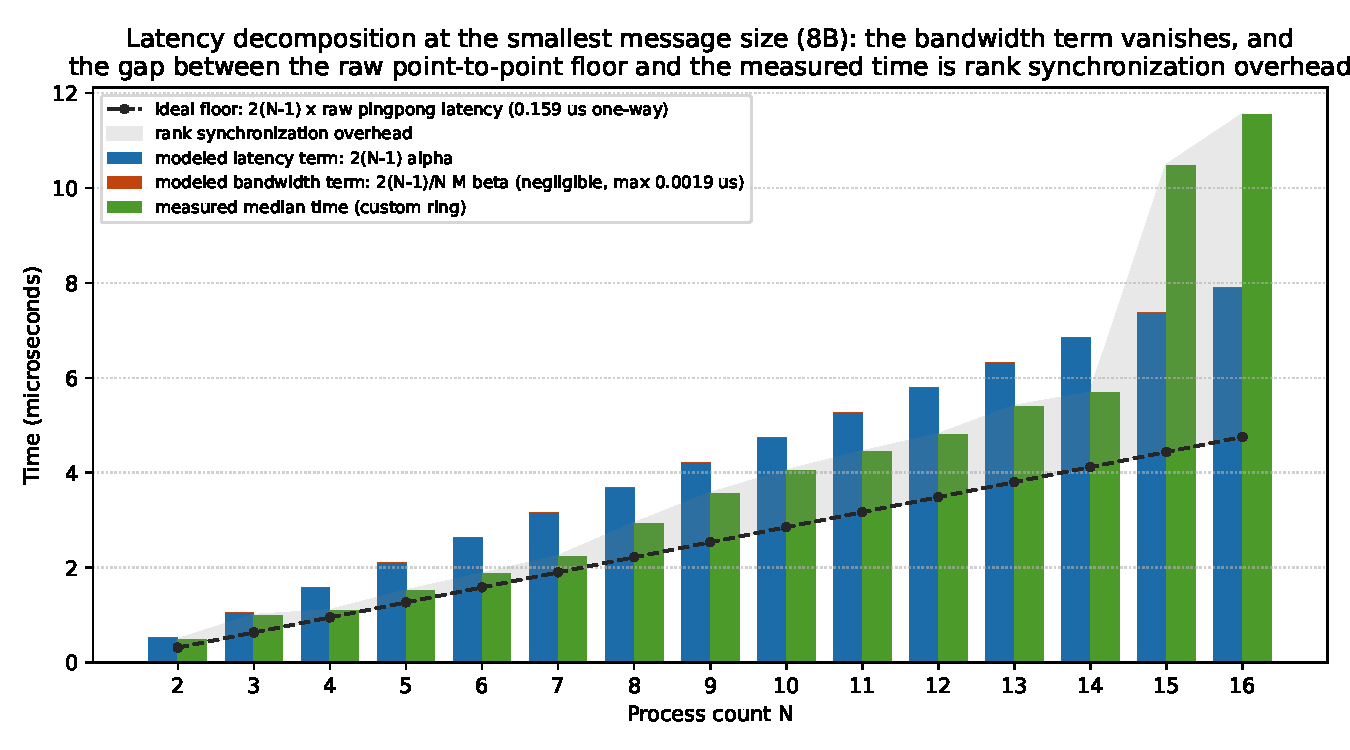
\includegraphics[width=\textwidth]{figures/latency_decomposition.pdf}
\caption{At the smallest swept message size (8~B), the ring's modeled latency term $2(N-1)\alpha$ and modeled bandwidth term $2\frac{N-1}{N}M\beta$ (the latter negligible, at most $0.0019~\mu$s), against the measured median time and against an ideal floor of $2(N-1)$ raw point-to-point latencies. The shaded gap between the floor and the measured time is rank synchronization overhead: near zero up to $N \approx 14$, then growing sharply.}
\label{fig:latency-decomposition}
\end{figure}
